% Integral de superficie: vector de área dσ = n̂ dσ (libro fig. 2.3)
\documentclass[border=4pt]{standalone}
\usepackage{tikz}
\usetikzlibrary{arrows.meta, calc}
\begin{document}
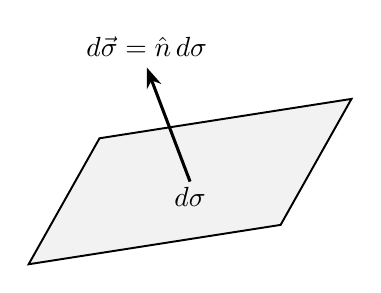
\begin{tikzpicture}[>={Stealth[length=2.6mm]}, line width=0.7pt]
  % parche de superficie (paralelogramo en perspectiva)
  \fill[black!5] (0,0) -- (3.2,0.5) -- (4.1,2.1) -- (0.9,1.6) -- cycle;
  \draw (0,0) -- (3.2,0.5) -- (4.1,2.1) -- (0.9,1.6) -- cycle;
  \node at (2.05,0.85){$d\sigma$};
  \coordinate (C) at (2.05,1.05);
  \draw[->, line width=1.1pt] (C) -- ($(C)+(-0.55,1.45)$) node[above]{$d\vec\sigma=\hat n\,d\sigma$};
\end{tikzpicture}
\end{document}
